

































\formatChapter{Pink Tag Boulders}
\phantomsection\label{sm:Pink Tag area map}
	\setbox0=\hbox{\begin{overpic}[width=0.8\linewidth]{./maps/area/out/Pink Tag_c.png}
	\end{overpic}}
	\needspace{\ht0}
	\begin{center}
	\begin{overpic}[width=0.9\linewidth]{./maps/area/out/Pink Tag_c.png}
	\end{overpic}
	\end{center}


\raggedcolumns
\begin{multicols}{2}
\qrcode{./maps/qr//Pink Tag Boulders_qr.png}{http://maps.google.com/maps?q=44.43998124232581,-122.57539325959186}{Navigate to this area}

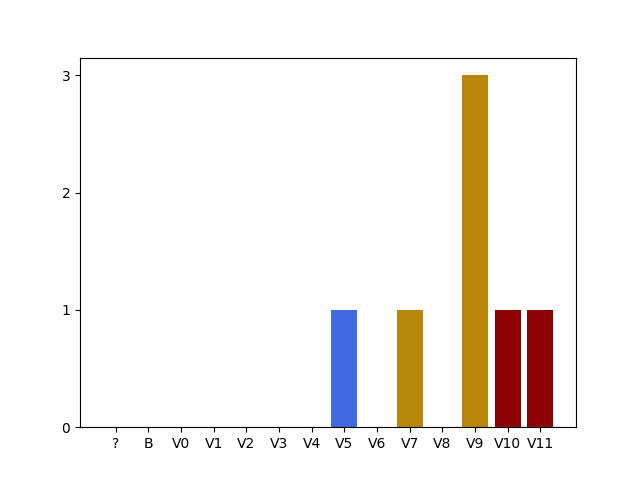
\includegraphics[width=\linewidth]{./maps/plots//Pink Tag Boulders.png}
\end{multicols}
\begin{multicols}{2}

Just across the road from the main area lay a few boulders on the banks of the River. Beware that at high flow rates most of the area will be underwater. Since the River is dam controlled the water level can shift rapidy. Consult the USGS flow charts for below green peter damn to know when the river will be low.

See driving directions for the Garden Main area.\\



\needspace{6em}
\phantomsection\label{pt:pinkTag}
	\setbox0=\hbox{\begin{overpic}[width=0.8\linewidth]{./images/pinkTagSign.jpg}\put (0,5) {\colorbox{\chapterColor}{\parbox{0.7\linewidth}{\textcolor{white}{Tread carefully, all but one of the climbs in this area are downhill of this sign.}}}}

	\end{overpic}}
	\needspace{\ht0}
	\begin{center}
	\begin{overpic}[width=0.9\linewidth]{./images/pinkTagSign.jpg}\put (0,5) {\colorbox{\chapterColor}{\parbox{0.7\linewidth}{\textcolor{white}{Tread carefully, all but one of the climbs in this area are downhill of this sign.}}}}

	\end{overpic}
	\end{center}






\phantomsection\label{tp:Territorial Pissings}
	\setbox0=\hbox{\begin{overpic}[width=0.8\linewidth]{./maps/topos/pissings_c.png}
	\end{overpic}}
	\needspace{\ht0}
	\begin{center}
	\begin{overpic}[width=0.9\linewidth]{./maps/topos/pissings_c.png}
	\end{overpic}
	\end{center}


\needspace{3em}
\subsection*{Pissing Boulder}\phantomsection\label{bf:Pissing Boulder}

This blunt overhanging corner is the first boulder that you walk by when entering Pink Tag.\\



\needspace{2em}
\phantomsection\label{rt:Territorial Pissings}
\colorbox{RoyalBlue!20}{
\parbox{0.95\linewidth}{
\hspace{-1ex}\textbf{$\Box$
1 Territorial Pissings V5*  
}}}
\begin{adjustwidth}{1.3em}{}			

PLACEHOLDER
\end{adjustwidth}




\phantomsection\label{tp:Jonah's Dab Rig}
	\setbox0=\hbox{\begin{overpic}[width=0.8\linewidth]{./maps/topos/jonah_c.png}
	\end{overpic}}
	\needspace{\ht0}
	\begin{center}
	\begin{overpic}[width=0.9\linewidth]{./maps/topos/jonah_c.png}
	\end{overpic}
	\end{center}


\needspace{3em}
\subsection*{Jonah's Dab Rig}\phantomsection\label{bf:Jonah's Dab Rig}




\needspace{2em}
\phantomsection\label{rt:Jonah's Dab Rig}
\colorbox{Goldenrod!20}{
\parbox{0.95\linewidth}{
\hspace{-1ex}\textbf{$\Box$
2 Jonah's Dab Rig V9 \ding{72}\ding{72} 
}}}
\begin{adjustwidth}{1.3em}{}			

Start standing in compression with left hand on a good sidepull and right hand on a blocky sloper, both near eye level. Crank a few powerful moves followed by several dabby moves climbing out of a small hole. Not dabbing is a significant contributor to the overall difficulty.
\end{adjustwidth}


\begin{adjustwidth}{0.5cm}{}				
\needspace{4em}
\textbf{Variations:} \newline

\needspace{2em}
\phantomsection\label{vr:Workshop 68}
\colorbox{red!20}{
\parbox{0.95\linewidth}{
\hspace{-1ex}\textbf{$\Box$
2a Workshop 68 V11*  
}}}
\begin{adjustwidth}{1.3em}{}			

PLACEHOLDER
\end{adjustwidth}



\end{adjustwidth}


\phantomsection\label{tp:Frat House}
	\setbox0=\hbox{\begin{overpic}[width=0.8\linewidth]{./maps/topos/fratHouse_c.png}
	\end{overpic}}
	\needspace{\ht0}
	\begin{center}
	\begin{overpic}[width=0.9\linewidth]{./maps/topos/fratHouse_c.png}
	\end{overpic}
	\end{center}


\needspace{3em}
\subsection*{Frat House}\phantomsection\label{bf:Frat House}




\needspace{2em}
\phantomsection\label{rt:Frat House}
\colorbox{green!20}{
\parbox{0.95\linewidth}{
\hspace{-1ex}\textbf{$\Box$
3 Frat House V2 \ding{72} \warn\warn
}}}
\begin{adjustwidth}{1.3em}{}			

Sit start with a juggy left hand sidepull and right hand meet hook on the corner of a low protrusion. Pull a few moves in compression before trending right to top over frat mouse. Climbing this with ample padding might recontextualize the star rating and the seriousness.
\end{adjustwidth}




\needspace{2em}
\phantomsection\label{rt:Frat Mouse}
\colorbox{green!20}{
\parbox{0.95\linewidth}{
\hspace{-1ex}\textbf{$\Box$
4 Frat Mouse V1 \ding{73} \warn
}}}
\begin{adjustwidth}{1.3em}{}			

Start on a flexing crack in the broken rock. Climb straight up using opposing sidepulls. The landing requires substantial padding to be made safe.
\end{adjustwidth}



\phantomsection\label{tp:Farley}
	\end{multicols}
	\setbox0=\hbox{\begin{overpic}[width=0.8\linewidth]{./maps/topos/farley_c.png}
	\end{overpic}}
	\needspace{\ht0}
	\begin{center}
	\begin{overpic}[width=0.9\linewidth]{./maps/topos/farley_c.png}
	\end{overpic}
	\end{center}
	\raggedcolumns
	\begin{multicols}{2}


\needspace{2em}
\phantomsection\label{rt:Belushi}
\colorbox{RoyalBlue!20}{
\parbox{0.95\linewidth}{
\hspace{-1ex}\textbf{$\Box$
5 Belushi V5/7* \ding{72}\ding{72} \warn
}}}
\begin{adjustwidth}{1.3em}{}			

Start matched in a threaded jug. Use all manner of trickery to pull the short roof and mantle your way to victory. Be careful even though the meat of this boulder is shorter than your average 8th grader the landing is uneven and swinging off the lip can send you tumbling towards the river (ask me how I know).
\end{adjustwidth}


\begin{adjustwidth}{0.5cm}{}				
\needspace{4em}
\textbf{Variations:} \newline

\needspace{2em}
\phantomsection\label{vr:Knowledge is Good}
\colorbox{Goldenrod!20}{
\parbox{0.95\linewidth}{
\hspace{-1ex}\textbf{$\Box$
5a Knowledge is Good V7*  
}}}
\begin{adjustwidth}{1.3em}{}			

Start as for Belushi and link into Lippity Split.
  (No Topo)
\end{adjustwidth}



\end{adjustwidth}


\needspace{2em}
\phantomsection\label{rt:Lippity Split}
\colorbox{RoyalBlue!20}{
\parbox{0.95\linewidth}{
\hspace{-1ex}\textbf{$\Box$
6 Lippity Split V5*  
}}}
\begin{adjustwidth}{1.3em}{}			

Start on the big horn at the far left of the lip and traverse right topping out above Farley Prep.
\end{adjustwidth}




\needspace{2em}
\phantomsection\label{rt:Le Lemét}
\colorbox{Goldenrod!20}{
\parbox{0.95\linewidth}{
\hspace{-1ex}\textbf{$\Box$
7 Le Lemét V9*  
}}}
\begin{adjustwidth}{1.3em}{}			

Sit start on jugs in the big pod climb up and right on thin edges.
\end{adjustwidth}




\needspace{2em}
\phantomsection\label{rt:Farley Prep}
\colorbox{Goldenrod!20}{
\parbox{0.95\linewidth}{
\hspace{-1ex}\textbf{$\Box$
8 Farley Prep V9*  
}}}
\begin{adjustwidth}{1.3em}{}			

Sit start with left hand on a small underclinging side pull and right hand on a lump on the arête. The lip is right there, how hard could it be?
\end{adjustwidth}






\end{multicols}
\clearpage